\section{Introduction}
\label{sec:introduction}

Modern AI systems are increasingly powered by Mixture-of-Experts
(MoE) language models such as DeepSeek-V3, Qwen3, Kimi-K2, and
GPT-OSS~\cite{deepseekai2025deepseekv3technicalreport,yang2025qwen3technicalreport,openai2025gptoss120bgptoss20bmodel,kimiteam2026kimik2openagentic},
whose training depends on systems that scale across distributed
clusters. Production frameworks~\cite{shoeybi2020megatronlmtrainingmultibillionparameter,narayanan2021efficientlargescalelanguagemodel,deepspeed,rajbhandari2020zeromemoryoptimizationstraining} have built end-to-end MoE
training stacks over years of engineering effort, pairing layered
Python designs with extra compiled extensions to deliver broad
model coverage, peak throughput, and multi-platform support
needed for diverse training workloads.
However, evolving these stacks for new model architectures and
system optimizations demands in-depth expertise and substantial
engineering effort.

AI coding agents~\cite{claude-code,codex-cli,cursor,github-copilot}
have begun to automate parts of this work and could in principle
accelerate training-system development. Most current practice
applies agents to existing frameworks. But the design choices
that helped human engineers cost agents differently. Plugin
systems, registry-based indirection, and heavy compiled extensions
raise the cost of locating relevant code, tracing what runs at a
given call site, and verifying a change is complete. Today's
throughput-only evaluations leave this cost unmeasured, and
existing frameworks were not designed with it in mind.

This raises a design question: \emph{can we redesign an MoE
training framework that optimizes for agent-task efficiency?} We
define \emph{agent-task efficiency} (ATE) as the cost of using
coding agents to understand, operate, and extend a framework,
measured along dimensions such as session duration and output
tokens. We
answer this question with \sys, an end-to-end MoE training
framework designed agent-native from the start. \sys is built on
four design principles. First, we favor code compactness over
coverage: \sys focuses on a compact MoE training stack rather than
the broad model and feature coverage of production frameworks,
while remaining straightforward for agents to extend with new
features.
Second, we use minimal, Python-native components covering the key
layers of MoE training: operators, training engine, and
applications. Third, we use direct calls and avoid implicit
indirection in module composition, so that what runs at a given
call site can be identified by static reading. Finally, we ship
agent skills~\cite{anthropic-skills} for recurring
training-framework tasks.

Beyond building the framework, we systematically evaluate how
framework design affects agent-task efficiency on real
training-system tasks. Existing AI-coding
benchmarks~\cite{jimenez2024swebench,chen2021evaluatinglargelanguagemodels,austin2021programsynthesislargelanguage}
vary the agent on a fixed codebase to score agent capability,
focusing on general software-engineering tasks such as issue
resolution. We invert this with \sysbench, a comprehensive benchmark that varies
the framework on real-world training-framework tasks, holding
the agent fixed so that differences in agent cost isolate
framework design. \autoref{fig:overview} summarizes \sys's
overall design.

\begin{figure}[!t]
  \centering
  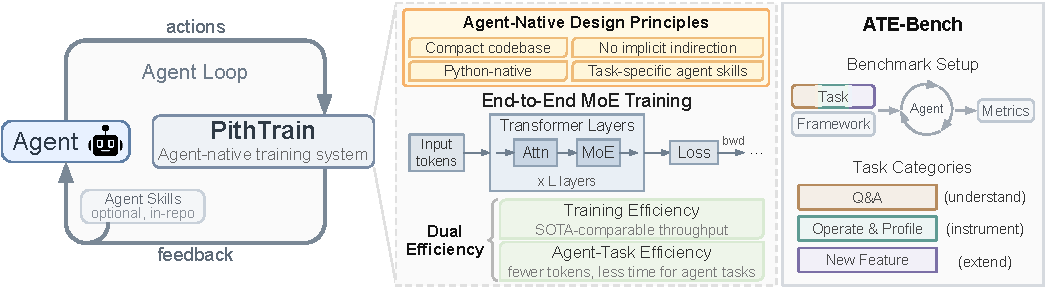
\includegraphics[width=0.95\textwidth]{figures/fig1_overview.pdf}
  \caption{\sys overview. An agent issues actions and consumes
  feedback (left); built on four agent-native design principles,
  \sys delivers dual efficiency (middle); \sysbench evaluates
  agent-task efficiency across frameworks (right).}
  \label{fig:overview}
\end{figure}

This paper makes three contributions:

\squishlist
    \item \textbf{\sys, a compact, Python-native, end-to-end MoE
    training framework.} A roughly 11K-line MoE training framework
    designed agent-native from the start, matching the training
    throughput of production frameworks.
    \vspace{-2pt}
    \item \textbf{Four design principles for agent-native ML
    training frameworks}, guiding \sys's design: code compactness,
    Python-native components, no implicit indirection, and agent
    skills.
    \vspace{-2pt}
    \item \textbf{Agent-task efficiency, \sysbench, and an
    empirical study.} Agent-task efficiency as a metric beyond
    training throughput, instantiated in \sysbench, with an
    empirical study showing
    \sys's higher agent-task efficiency over production frameworks,
    plus a skills ablation and case study.
\squishend

\sys delivers \emph{dual efficiency}: strong training throughput
together with high agent-task efficiency. It matches the throughput
of production frameworks across a range of MoE models and
training settings on NVIDIA H100 and B200 GPUs. On \sysbench, a
coding agent completes the same training-framework tasks on
\sys with up to 62\% fewer Agent Turns and 64\% less
Active GPU Time than on production frameworks
for the hardest new-feature tasks, with
similar reductions on other metrics. A qualitative case
study illustrates how framework design
shapes agent behavior.

